\documentclass[serif, aspectratio=169]{beamer}
\usepackage[T1]{fontenc} 
\usepackage{fourier}
\usepackage{hyperref}
\usepackage{latexsym,amsmath,xcolor,multicol,booktabs,calligra}
\usepackage{booktabs} % For better table formatting
\usepackage{graphicx,pstricks,listings,stackengine}
\usepackage{listings}
\usepackage{array} 
\usepackage{colortbl}

\author{Dr.Hajialiasgari}
\title{Machine Learning}
\institute{
    Tehran University \\
    Of\\
    Medical Science
}
\date{\small \today}
\usepackage{UoWstyle}

% Define custom colors and styles for listings
\definecolor{deepblue}{rgb}{0,0,0.5}
\definecolor{deepred}{RGB}{153,0,0}
\definecolor{deepgreen}{rgb}{0,0.5,0}
\definecolor{halfgray}{gray}{0.55}

\lstset{
    basicstyle=\ttfamily\small,
    keywordstyle=\bfseries\color{deepblue},
    emphstyle=\ttfamily\color{deepred},
    stringstyle=\color{deepgreen},
    numbers=left,
    numberstyle=\small\color{halfgray},
    rulesepcolor=\color{red!20!green!20!blue!20},
    frame=shadowbox,
}

\begin{document}

\begin{frame}
    \titlepage
    \vspace*{-0.6cm}
    \begin{figure}[htpb]
        \begin{center}
            \includegraphics[keepaspectratio, scale=0.05]{Tumsl-logo.png}
        \end{center}
    \end{figure}
\end{frame}

\begin{frame}    
\tableofcontents[sectionstyle=show, subsectionstyle=show/shaded/hide, subsubsectionstyle=show/shaded/hide]
\end{frame}

\section{Data Preparation}

\section{Introduction to Data in Machine Learning}
\begin{frame}
    \begin{itemize}
        \item Data is a crucial component in the field of Machine Learning. It refers to the set of observations or measurements that can be used to train a machine-learning model. 
        \item The quality and quantity of data available for training and testing play a significant role in determining the performance of a machine-learning model. Data can be in various forms such as numerical, categorical, or time-series data, and can come from various sources such as databases, spreadsheets, or APIs. Machine learning algorithms use data to learn patterns and relationships between input variables and target outputs, which can then be used for prediction or classification tasks.
    \end{itemize}
\end{frame}

\begin{frame}{Transformation of Data}
    \centering
    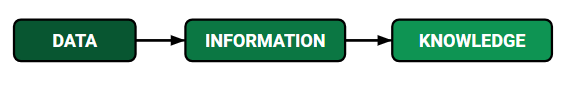
\includegraphics[width=0.8\textwidth]{DATA-1.png}
\end{frame}

\section{Questions About Data}

\begin{frame}
    \begin{itemize}
        \item \texttt{\color{red}Can the desired data be accessed?}\newline Before using data, ensure it is accessible, complies with legal, ethical, and financial considerations, and check for any agreements needed with data owners. Handle sensitive data carefully, removing personal identifiers when sharing. Consult legal experts to avoid future issues.
        \item \texttt{\color{red}Is the data volume sufficient?}\newline In machine learning, the required data volume is often uncertain, especially with strict performance criteria. Consider how quickly new data is generated—start with existing data, and allow new data to flow in during feature engineering, modeling, or other tasks. Use a representative subset for efficient training, and ensure it reflects the overall dataset characteristics.
    \end{itemize}
\end{frame}

\begin{frame}
    \begin{itemize}
        \item \texttt{\color{red}Is the data usable?} 
        \item Data  quality significantly affects model performance. Ensure the dataset is real, appropriately formatted (rows as samples, columns as features), and free of missing or duplicate values unless intended. Outdated data can limit model relevance, and incomplete datasets may lack diversity, affecting generalization.
        \item For example, the dataset might only include animals from a specific geographical region or images taken in a particular season, making it less representative of real-world scenarios.
    \end{itemize}
\end{frame}

\begin{frame}
    \begin{itemize}
        \item \texttt{\color{red}Is the data understandable?} 
        \item If the dataset is not fully understood, it can lead to errors during modeling. For instance, if the target variable is entirely calculable using one of the dataset features, but you are unaware of this relationship, it may result in misleading outcomes.
    \end{itemize}
\end{frame}

\begin{frame}
    \begin{itemize}{Data Leakage}
        \item Consider working on a house price prediction project where the model uses features like area, number of bedrooms, and neighborhood type. If you inadvertently include a feature like the real estate agent's commission—which has a direct relationship with the house price—this can cause \texttt{\color{red}data leakage}. The model might achieve near-perfect accuracy during training by exploiting this feature, but it will fail in real-world applications where such information isn’t available beforehand. Understanding the dataset thoroughly is essential to avoid such pitfalls..
    \end{itemize}
\end{frame}

\begin{frame}
    \begin{itemize}
        \item \texttt{\color{red}Is the data reliable?} 
        \item The reliability of data depends on the processes used for its collection. For instance, if labels are assigned by unwilling individuals or collected through sensors of questionable accuracy, their trustworthiness is debatable.

        \item Data reliability is also affected by delayed or indirect labeling. In delayed labeling, such as predicting customer retention 6 months ahead based on current behavior, significant intervening events may reduce label reliability. Indirect labeling, like inferring user interest in Instagram pages through actions like clicks or likes, can be misleading due to errors or external influences like advertisements. Ensuring data reliability is crucial for robust model performance.
    \end{itemize}
\end{frame}

\section{Data Challenges}


\begin{frame}{Labeling Samples}
    \begin{itemize}
        \item n supervised learning, labeled datasets are essential, but most available datasets are unlabeled. Consequently, a significant portion (around 80\%) of machine learning project time is spent collecting, organizing, and labeling data. Since manual labeling is resource-intensive, many teams rely on pre-labeled datasets.

        \item  example, to map business types in a city, buying data from a government body might be impractical due to incomplete or outdated records. Alternatively, you could collect images using camera-equipped vehicles and manually label businesses (e.g., cafés, gyms, pharmacies), though this approach is costly.

        \item Creative solutions include using software to streamline labeling or leveraging semi-supervised learning—manually label a small dataset to train a basic model and use it to label the rest, verified by human reviewers. This reduces the labeling burden significantly.

    \end{itemize}
\end{frame}


\begin{frame}{Data Quality}
    \begin{itemize}
        \item The quality of the dataset is one of the factors affecting model performance and consists of two main components:
        \item \texttt{\color{red}Raw Dataset Quality}
        \item \texttt{\color{red}Labeling Quality}
    \end{itemize}
\end{frame}

\begin{frame}
    \begin{itemize}
        \item Some common issues in raw datasets include the following, with some explained in this lesson and the last two covered in detail in future lessons:
        \item \texttt{\color{red}Noise}
        \item \texttt{\color{red}Bias}
        \item \texttt{\color{red}Low predictive power}
        \item \texttt{\color{red}Obsolescence}
         \item \texttt{\color{red}Outliers}
        \item \texttt{\color{red}Data Leakage}
    \end{itemize}
\end{frame}

\begin{frame}{Noise}
    \begin{itemize}
        \item A "noise" refers to a distorted or unrealistic sample. For example, a portion of an image may be missing, making it a noisy sample. Words in a text may be merged or improperly spaced, or there could be noise in audio data and similar issues. These types of data can often be partially corrected, such as recovering damaged images using specific algorithms. The problem of noisy data becomes more significant when the number of training samples is small (thousands or fewer). In such cases, noisy data can mislead the model's learning process. For instance, if there are 1,000 samples ranging between 0 and 10, along with three noisy samples exceeding 1,000, these three outliers can significantly skew the dataset's mean and variance.
    \end{itemize}
\end{frame}

\begin{frame}{Bias}
    \begin{itemize}
        \item Some common issues in raw datasets include the following, with some explained in this lesson and the last two covered in detail in future lessons:
        \item \texttt{\color{red}Noise}
        \item \texttt{\color{red}Bias}
        \item \texttt{\color{red}Low predictive power}
        \item \texttt{\color{red}Obsolescence}
         \item \texttt{\color{red}Outliers}
        \item \texttt{\color{red}Data Leakage}
    \end{itemize}
\end{frame}




\begin{frame}
    \begin{center}
        {\Huge\ End of Data Preparation}
    \end{center}
\end{frame}

\end{document}

